% !Mode:: "TeX:UTF-8:Hard"
\documentclass{beamer}
\usepackage[UTF8,indent]{ctexcap}
\usetheme{Madrid}%Madrid,JuanLesPins,Ilmenau
\usefonttheme[onlymath]{serif}

\newcommand\Emph{\textbf}

\AtBeginSection[]{
  \begin{frame}
  \vfill
  \centering
  \begin{beamercolorbox}[sep=8pt,center,shadow=true,rounded=true]{title}
    \usebeamerfont{title}\insertsectionhead\par%
  \end{beamercolorbox}
  \vfill
  \end{frame}
}

\AtBeginSubsection[]{
  \begin{frame}
  \vfill
  \centering
  \begin{beamercolorbox}[sep=8pt,center,shadow=true,rounded=true]{title}
    \usebeamerfont{title}\insertsubsectionhead\par%
  \end{beamercolorbox}
  \vfill
  \end{frame}
}

\AtBeginSubsubsection[]{
  \begin{frame}
  \vfill
  \centering
  \begin{beamercolorbox}[sep=8pt,center,shadow=true,rounded=true]{title}
    \usebeamerfont{title}\insertsubsubsectionhead\par%
  \end{beamercolorbox}
  \vfill
  \end{frame}
}


\title{面向节能的单/多列车优化决策问题}
%\author{三峡大学\and 艾鑫\\ 武汉大学\and 杨志巧\\ 湖南大学\and 李金武}

\author[艾鑫、杨志巧、李金武]{艾鑫 \inst{1} \and 杨志巧 \inst{2} \and 李金武 \inst{3}}
\institute[三大、武大、湖大]{\inst{1} 三峡大学\hspace{1em}理学院 \and %
                      \inst{2} 武汉大学\hspace{1em}数学与统计学院 \and %
                      \inst{3} 湖南大学\hspace{1em}机械与运载工程学院}

\date{\today}

\begin{document}
\maketitle

\section{问题回顾}
\subsection{第一问、单列车节能运行优化控制问题}
\begin{frame}{问题回顾}{问题一、单列车节能运行优化控制问题}
\begin{description}
  \item[第一小问] 请建立计算速度距离曲线的数学模型,计算寻找一条列车从$A_6$站出发到
达$A_7$站的最节能运行的速度距离曲线,其中两车站间的运行时间为110秒
  \item[第二小问] 请建立新的计算速度距离曲线的数学模型,计算寻找一条列车从$A_6$站出
发到达$A_8$站的最节能运行的速度距离曲线,其中要求列车在$A_7$车站停站45秒,$A_6$站和$A_8$站间
总运行时间规定为220秒(不包括停站时间)
\end{description}
\end{frame}

\subsection{第二问、多列车节能运行优化控制问题}
\begin{frame}{问题回顾}{第二问、多列车节能运行优化控制问题}
\begin{description}
  \item[第一小问] 当100列列车以间隔$H={h_1,\cdots,h_{99}}$从$A_1$站出发,\Emph{追踪运行},依次经
  过$A_2$,$A_3$,……到达$A_{14}$站,中间在各个车站停战最少$D_{\min}$秒,最多$D_{\max}$秒。间隔$H$各
  分量的变化范围是$H_{\min}$秒至$H_{\max}$秒。请建立优化模型并寻找使所有列车运行总能耗最低的间隔H。
  要求第一列列车发车时间和最后一列列车的发车时间之间间隔为$T_0=63900$秒,且从$A_1$站到$A_{14}$站的
  总运行时间不变,均为$2086$秒(包括停站时间)。假设所有列车处于同一供电区段。
\end{description}
\end{frame}

\begin{frame}{问题回顾}{第二问、多列车节能运行优化控制问题}
\begin{description}
  \item[第二小问] 接上问,如果高峰时间(早高峰$7200$秒至$12600$秒,晚高峰$43200$至$50400$秒)发车间隔
  不大于$2.5$分钟且不小于$2$分钟,其余时间发车间隔不小于$5$分钟,每天$240$列。请重新为它们制定运行图和相应
  的速度距离曲线。
\end{description}
\end{frame}

\subsection{第三问、列车延误后运行优化控制问题}
\begin{frame}{问题回顾}{第三问、列车延误后运行优化控制问题}
\begin{description}
  \item[第一小问] 接上问,若列车$i$在车站$A_j$延误$DT_j^i$(10秒)发车,请建立控制模型,找出在确保安全的前提下,首先使所有后
续列车尽快恢复正点运行,其次恢复期间耗能最少的列车运行曲线
  \item[第二小问] 假设$DT_j^i$为随机变量,普通延误($0<DT_j^i <10 \, \mathrm{s}$)概率为$20\%$,严重延误($DT_j^i >10 \, \mathrm{s}$)概率为$10\%$(超
过$120$秒,接近下一班,不考虑调整),无延误($DT_j^i= 0$)概率为$70\%$。若允许列车在各站到、发时间与原时
间相比提前不超过$10$秒,根据上述统计数据,如何对第二问的控制方案进行调整?
\end{description}
\end{frame}

\section{问题求解}
\subsection{第一问、单列车节能运行优化控制问题}
\subsubsection{模型建立}
\begin{frame}{目标函数的确定}
题设给出的目标是使得耗能最少,根据题设可知耗能主要是由于列车行驶需要牵引力,导致发电机就处于耗能状
态。查阅相关参考文献[2]可知在整个运行过程中所消耗的能量由牵引力来决定,如下所示:
\[E = \int_0^{{t_{\max }}} {F\left( t \right){v_t}dt} \]

注:${t_{\max }} = 110$ ,因为总的运行时间为110 秒。
\end{frame}

\begin{frame}{约束条件的确定}
约束条件一:由题目所给的数据中可以知道从 $A_6$站到 $A_7$站的总路程为1354m,因此整个过程中行走的总路程${L_{\max }} = 1354$ m,即:
\[\int_o^{{t_{\max }}} {{v_t}dt}  = {L_{\max }}\]
\\
约束条件二:列车起始时刻和到达 $A_7$站时刻的速度均为0且在运行的任何时刻速度都不能大于该时刻所处路段的最大速度$\overline {{v_t}} $ ,即:
\[\left\{ \begin{array}{l}
 {v_0} = {v_{{t_{\max }}}} = 0 \\
 {v_t} \le \overline {{v_t}}  \\
 \end{array} \right.\]
\\
约束条件三:由牛顿学第二定律可知,实际输出的牵引加速度乘以质量等于合外力,即:
\[m{a_t} = m\frac{{d{v_t}}}{{dt}} = F\left( t \right) - B\left( t \right) - W\left( t \right)\]
\end{frame}

\begin{frame}{第一问模型}
 综上所述,建立的单列车两个站点之间的最优化模型为:
\[\min {\kern 1pt} {\kern 1pt} {\kern 1pt} {\kern 1pt} {\kern 1pt} {\kern 1pt} {\kern 1pt} {\kern 1pt} {\kern 1pt} {\kern 1pt} E = \int_o^{{t_{\max }}} {F\left( t \right){v_t}dt} \]
\[s.t.\left\{ \begin{array}{l}
 \int_o^{{t_{\max }}} {{v_t}dt}  = {L_{\max }} \\
 \left\{ \begin{array}{l}
 {v_0} = {v_{{t_{\max }}}} = 0 \\
 {v_t} \le \overline {{v_t}}  \\
 \end{array} \right. \\
 m{a_t} = m\frac{{d{v_t}}}{{dt}} = F\left( t \right) - B\left( t \right) - W\left( t \right) \\
 F\left( t \right) = {k_t}{F_{\max }}\left( t \right) \\
 B\left( t \right) = {k_b}{B_{\max }}\left( t \right) \\
 W\left( t \right) = \left[ {{w_0}\left( t \right) + {w_1}\left( t \right)} \right] \times g \times {m \mathord{\left/
 {\vphantom {m {1000}}} \right.
 \kern-\nulldelimiterspace} {1000}} \\
 \end{array} \right.\]

\end{frame}

\subsubsection{求解算法}
\begin{frame}{换一个角度看问题}

\begin{itemize}
  \item<1-> 题目要求在给定的时间内,使消耗的能量最小
  \item<2-> 给定时间让能量最小$\Longrightarrow$ 比较困难
  \item<3-> 给定能量让时间最小$\Longrightarrow$ 容易求解
  \item<4-> 可以将第一个问题转化为第二个问题,首先构造一个能量比较小的初始解,然后不断的增加能量,直到时间
  满足要求
\end{itemize}
\end{frame}

\begin{frame}{为什么能够这么做?}
    \begin{columns}[c]
        \column{8cm}
            \begin{itemize}
              \item 将此问题推广为一个多目标规划问题
                \begin{itemize}
                  \item 目标一:$\min \quad t$
                  \item 目标二:$\min \quad E$
                \end{itemize}
              \item 运行方案$(t,E) \Longrightarrow  P(t,E)$
              \item 多目标规划:Pareto front $C$(非劣解集)
            \end{itemize}
        \column{5cm}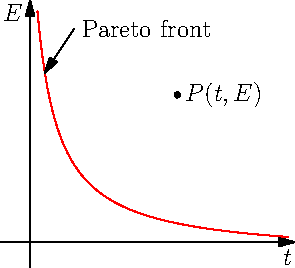
\includegraphics[width=4.5cm]{fig/fig1/fig1.pdf}
    \end{columns}
\end{frame}

\begin{frame}{为什么能够这么做?}
    \begin{columns}[c]
        \column{8cm}
            \begin{itemize}
              \item 原问题:给定时间$t_n$,求$E_{\min}$ $\Longrightarrow$ 求$t = t_n$与$C$的交点对应的运行方案
              \item 如果我们能够给出能量较小的初始解$(t_1,E_1)$,然后逐步添加能量,直到$t = t_n$,即求得原问题的运行方案
            \end{itemize}
        \column{5cm}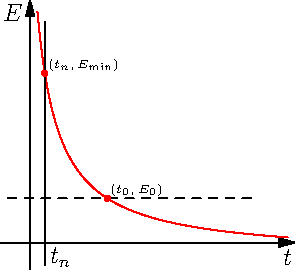
\includegraphics[width=4.5cm]{fig/fig2/fig2.pdf}
    \end{columns}
\end{frame}

\begin{frame}{为什么能够这么做?}
    \begin{columns}[c]
        \column{8cm}
            \begin{itemize}
              \item 原问题:给定时间$t_n$,求$E_{\min}$ $\Longrightarrow$ 求$t = t_n$与$C$的交点
              \item 如果我们能够给出能量较小的初始解$(t_1,E_1)$,然后逐步添加能量,直到$t = t_n$
            \end{itemize}
        \column{5cm}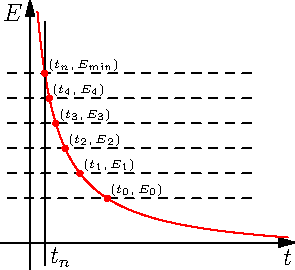
\includegraphics[width=4.5cm]{fig/fig3/fig3.pdf}
    \end{columns}
\end{frame}

\begin{frame}{考虑一个理想的情况}
\begin{columns}[c]
    \column{5cm}
        下面考虑一个理想的情况,即假设:
        \begin{itemize}
          \item 速度限制$v_{\max}$为常数
          \item 阻力$r$也为常数
        \end{itemize}
    \column{6cm}
    \begin{block}{优化模型}
        \begin{equation*}
          \min \quad E = \int_0^{t_{\max}} k_t(t) v(t) F(t) dt
        \end{equation*}
        \begin{equation*}
          s.t. \left\{
          \begin{array}{l}
            m \frac{dv(t)}{dt} = k_t F - k_b B - r \\
            L = \int_0^{t_{\max}} v(t) dt \\
            v(0) = v_0, \quad v(t_{\max}) = v_T \\
            k_t \in [0, 1], k_b \in [0,1], v \leq v_{\max}
          \end{array}
          \right.
        \end{equation*}
    \end{block}
\end{columns}
\end{frame}

\begin{frame}{Pontryagin最大值原理}
\begin{columns}[c]
    \column{6.5cm}
        根据Pontryagin最大值原理,前述优化模型可以转化为最大化下面的哈密顿函数:
        \begin{equation*}
          H = \frac{p_1}{v} \times (k_t F - k_b B - r) + p_2 v - k_t v F
        \end{equation*}
        其中$p_1$应该满足下面的微分方程:
        \begin{equation*}
          \frac{dp_1}{ds} = - \frac{\partial H}{\partial v}
        \end{equation*}
    \column{5.5cm}
    \begin{block}{求解结果}
    \begin{equation*}
      \left\{
        \begin{array}{l}
        k_t = 1, k_b = 0, \, (p_1>v^2) \\
        k_t \in [0,1], k_b = 0, \, (p_1 = v^2) \\
        k_t = 0, k_b \in [0,1], \, (p_1 = 0) \\
        k_t = 0, k_b = 0, \, (0 < p_1 < v^2) \\
        k_t = 0, k_b = 1, \, (p_1 < 0).
        \end{array}
      \right.
    \end{equation*}
    \end{block}
\end{columns}
\end{frame}

\begin{frame}{Pontryagin最大值原理}
\begin{columns}[c]
\column{5cm}
求解结果与四个阶段相对应:
\begin{description}
  \item[最大加速] $k_t = 1, k_b = 0$
  \item[巡航] $k_t \in [0,1], k_b = 0$
  \item[巡航] $k_t = 0, k_b \in [0,1]$
  \item[惰行] $k_t = 0, k_b = 0$
  \item[最大加速] $k_t = 0, k_b = 1$
\end{description}

\column{7cm} 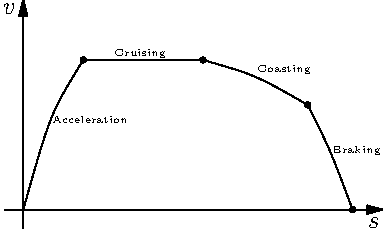
\includegraphics[width=7cm]{fig/fig4/fig4.pdf}
\end{columns}
\end{frame}

\end{document}
